\section{Case study}
Trong phần này, chúng ta sẽ cùng xem xét tình huống thực tế mà tác giả đã sử dụng ELK stack để theo dõi và cải thiện một ứng dụng điểm danh bằng khuôn mặt. Tính năng cốt lõi của ứng dụng là nhận vào một hình ảnh khuôn mặt được truyền từ thiết bị di động và tìm kiém trong cơ sở dữ liệu thông tin của ảnh đó. Thông tin trả ra là một ID mà sẽ được dùng để tham chiếu tới thông tin cá nhân của người điểm danh. Nếu tìm thấy ảnh trong cơ sở dữ liệu (điểm trên một ngưỡng nào đó), ứng dụng sẽ ghi ra một dòng log có dạng "\texttt{reid\_data: ReidMessage(msg='success', score=0.8236697316169739)}". Ngược lại, khi độ đo score dưới ngưỡng (có thể coi là không tìm thấy ảnh trong cơ sở dữ liệu), log có dạng "\texttt{reid\_data: ReidMessage(msg='cannot identify', 
 \\ score=0.2316697316169739)}". 

 \begin{figure}[H] % places figure environment here   
    \centering % Centers Graphic
    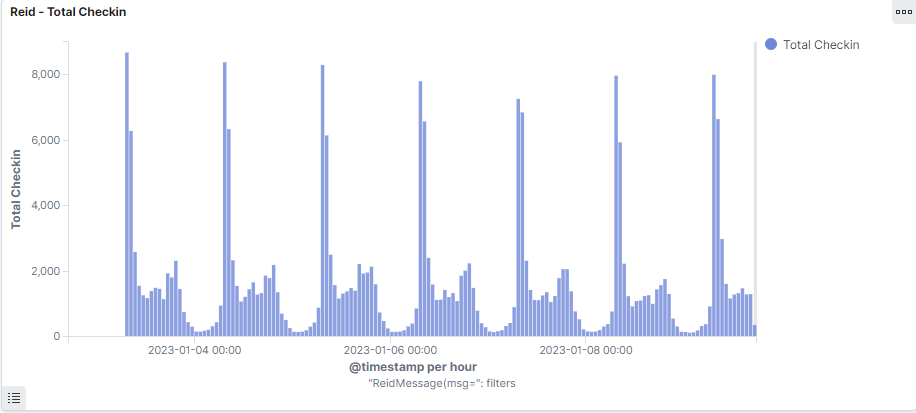
\includegraphics[width=1\textwidth]{figures/total_checkin.png} 
    \caption{Log điểm danh trong 7 ngày gần nhất} % Creates caption underneath graph
    \label{fig:elk_01}
\end{figure}

Với khả năng tìm kiếm full text mạnh mẽ của Elasticsearch, chúng ta có thể áp dụng bộ lọc lấy ra những log có chứa cụm từ "\texttt{ReidMessage(msg=}" nghĩa là bao trùm cả trường hợp điểm danh thành công hoặc thất bại, hay nói cách khác chính là log điểm danh mà hệ thống ghi nhận được. Tương tự như vậy ta có thể lọc ra những log chứa cụm từ "\texttt{ReidMessage(msg='cannot identify'}" để lấy ra các log điểm danh thất bại và trực quan hoá với biểu đồ dưới đây. Do dữ liệu là dạng dữ liệu hướng thời gian nên tác giả chọn biểu diễn bằng biểu đồ cột. Ngoài ra ta cũng có thể giữ chuột tại một vị trí nào đó để biết số lượng điểm danh (thất bại) trong một khung thời gian. Khoảng thời gian hoàn toàn có thể được tuỳ chỉnh một cách dễ dàng với thanh điều khiển của Kibana.

\begin{figure}[H] % places figure environment here   
    \centering % Centers Graphic
    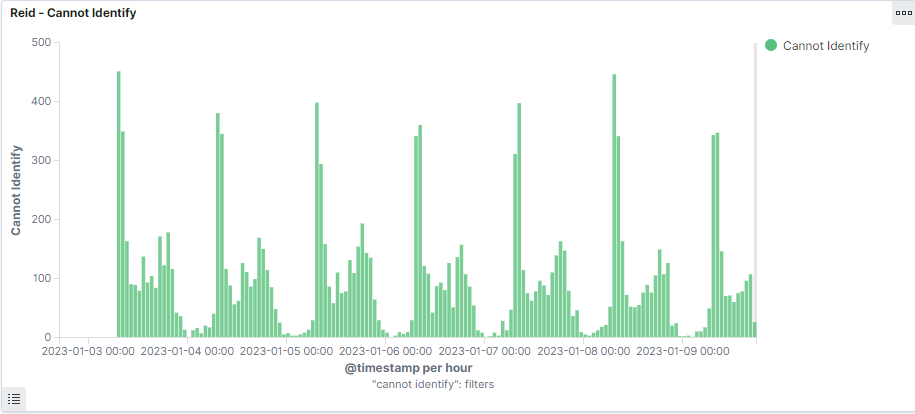
\includegraphics[width=1\textwidth]{figures/cannot_identify.png} 
    \caption{Log điểm danh thất bại trong 7 ngày gần nhất} % Creates caption underneath graph
    \label{fig:elk_01}
\end{figure}

\begin{figure}[H] % places figure environment here   
    \centering % Centers Graphic
    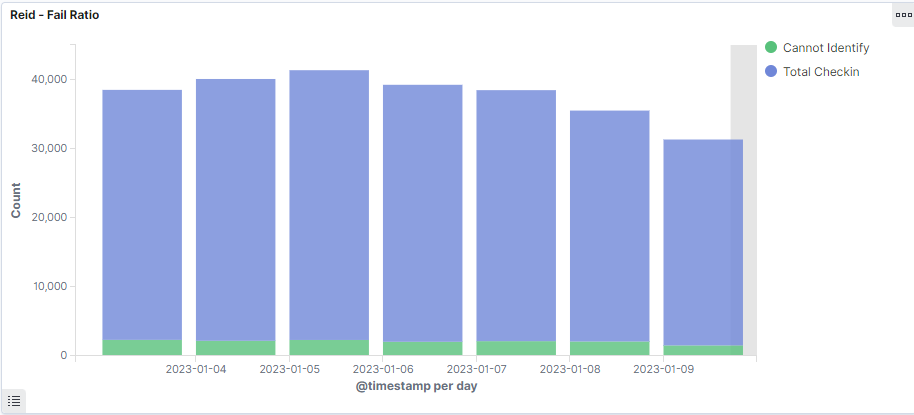
\includegraphics[width=1\textwidth]{figures/fail_ratio.png} 
    \caption{Tỉ lệ điểm danh thất bại trên tổng log điểm danh trong 7 ngày gần nhất} % Creates caption underneath graph
    \label{fig:elk_01}
\end{figure}

Quan sát biểu đồ, ta có thể nhận thấy số khung giờ cao điểm là khoảng 7 đến 8 giờ sáng và 17 đến 19 giờ tương ứng với thời điểm checkin và checkout của nhân viên. Ban đêm hầu như không có log điểm danh. Tỉ lệ điểm danh lỗi hàng ngày vào khoảng 6-8\%. Câu hỏi đặt ra là liệu người làm ứng dụng có thể làm tốt hơn? Đôi khi vài phần trăm không phải là vấn đề lớn trong tính toán nhưng với những nhân viên thường xuyên điểm danh thất bại hoặc thời gian điểm danh lâu thì đó là một trải nghiẹm rất tệ và ảnh hưởng trực tiếp tới ngày công của họ. 

\begin{figure}[H] % places figure environment here   
    \centering % Centers Graphic
    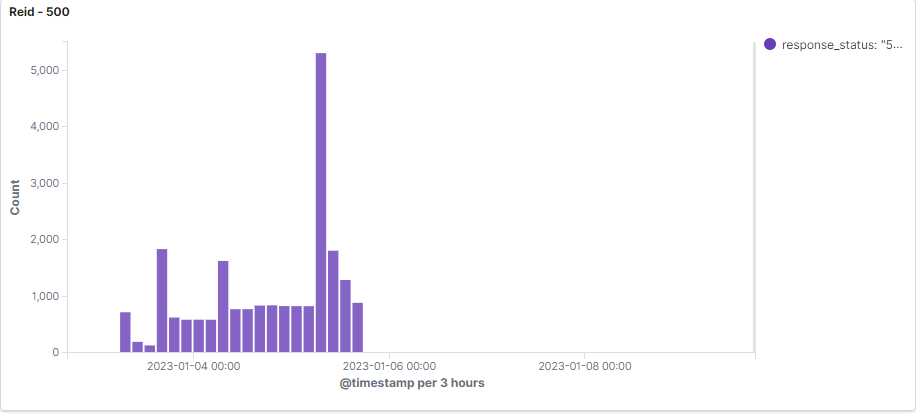
\includegraphics[width=1\textwidth]{figures/log-500.png} 
    \caption{Lỗi 500 xảy ra trong hệ thống} % Creates caption underneath graph
    \label{fig:elk_01}
\end{figure}

Và đây là điều bất ngờ khi tác giả biểu diễn số request bị lỗi 500. Như đã nói ở phần trước, lỗi phản hồi HTTP 500 là một lỗi nghiêm trọng vì chúng ta ...không biết nguyên nhân của nó! Ngay khi vừa vẽ biểu đồ biểu diễn số lượng lỗi 500, chúng tôi đã vô cùng hoang mang vì trước nay tất cả đều tưởng ứng dụng đang chạy ...tốt! Khi quan sát các biểu đồ trên và xếp kề theo một trục thẳng đứng, chúng ta thấy có một sự trùng hợp đó là thời điểm số log lỗi 500 trùng với thời điểm cao tải điểm danh. Tiếp tục truy vết và nghiên cứu code chúng tôi phát hiện ra rằng, khi có quá nhiều request vào hệ thống, ứng dụng bị nghẽn! Khi đó ứng dụng không thể tiếp nhận thêm yêu cầu và trả ra lỗi 500. Vậy là sau vài giây đứng chờ người dùng sẽ nhận được thông báo điểm danh thất bại. Đây quả thực là một trải nghiệm tệ. 

Để cải thiện, ban đầu, giải pháp được đưa ra là tăng phần cứng lên, ghép hêm CPU, GPU và tăng số lượng instances của ứng dụng. Nhưng chúng ta đều biết đây là phương án rất đắt đỏ bởi GPU là phần cứng không hề rẻ tiền và không sẵn có. Cuối cùng chúng tôi nghiên cứu code và chỉnh sửa và đây là kết quả. Số lỗi từ đỉnh trên 5000 ngày hôm trước còn dưới 10 vào ngày hôm sau!

\begin{figure}[H] % places figure environment here   
    \centering % Centers Graphic
    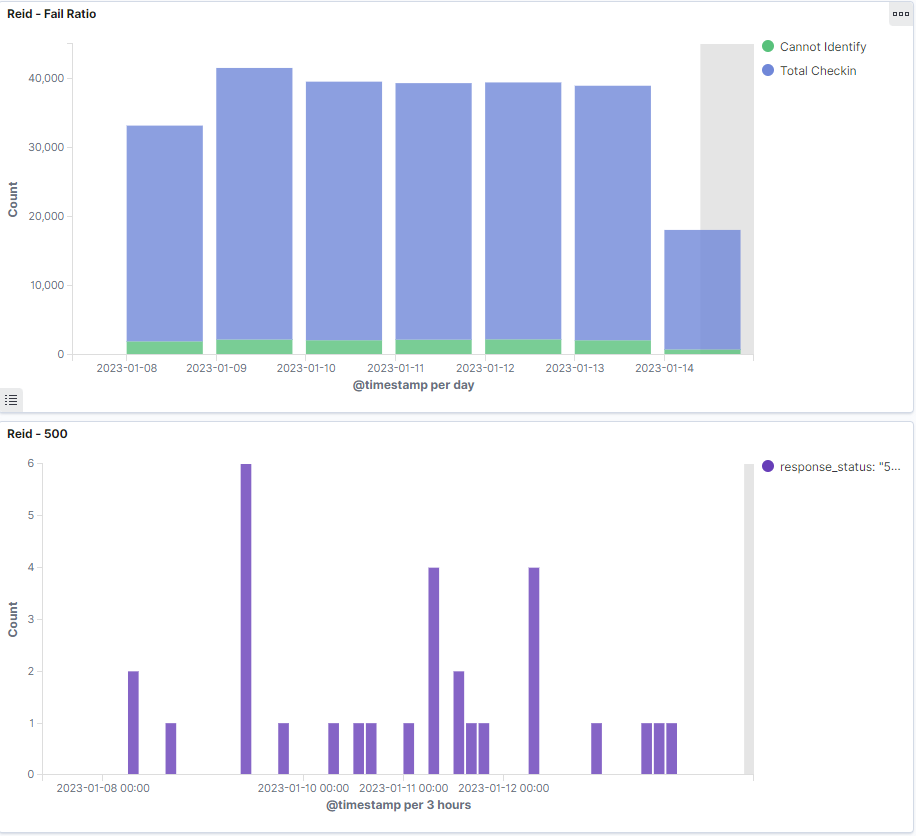
\includegraphics[width=1\textwidth]{figures/total_checkin_and_500.png} 
    \caption{Lỗi 500 xảy ra trong hệ thống sau khi sửa code} % Creates caption underneath graph
    \label{fig:elk_01}
\end{figure}

Chỉ bằng những biểu diễn trực quan hết sức ...thô sơ chúng tôi đã phát hiện lỗi và cải thiện ứng dụng một cách nhanh chóng và mang lại lợi ích đáng kể (thay vì phải mua thêm khoảng 4 GPU trị giá khoảng gần 200 triệu đồng). 

